\documentclass[french, 11pt]{report}
\usepackage[utf8]{inputenc}
\usepackage[T1]{fontenc}
\usepackage[a4paper]{geometry}
\usepackage{lmodern}
\usepackage{xcolor}
\usepackage{graphicx}
\usepackage{textcomp}
\usepackage[french]{babel}
\usepackage[breaklinks]{hyperref}
\usepackage{colortbl}

\title{Cahier des charges\\ Projet Licence 3 - Space Wars}
\date{Date de rédaction: \today}
\author{Tony Deborguere \\ Baris Tekeli \\ Malik Touat \\ Qi Zhiwen}

\begin{document}
	\maketitle
	\tableofcontents	
	
	\chapter{Présentation du projet}
	\begin{table}[h]
		\begin{center}
			\centering
			\begin{tabular}{llr}
				\hline\hline
				\rowcolor[RGB]{125,12,125}\multicolumn{3}{c}{\textcolor{white}{Fiche d'identité du projet}}\\\hline\hline
				Nom du projet: & Space Wars &\\\hline
				Objet: & \multicolumn{2}{l}{Création d'un clone de Space Invaders avec une partie Player Versus}\\
				& Player en réseaux. &\\\hline
				Membres du projet: & DEBORGUERE TONY & (t.deborguere@gmail.com) \\
				&TEKELI BARIS & (tekelibaris@gmail.com) \\
				&TOUAT MALIK & (mal.touat@gmail.com) \\
				&QI ZHIWEN & (531940615@qq.com) \\\hline
				Commanditaire: & JULIEN DEHOS &\\\hline
				Date de début: & 06 Juin 2016 &\\\hline
				Date de fin: & 22 Juin 2016 &\\\hline\hline
			\end{tabular}
		\end{center}
	\end{table}
	
	\section{Règle du jeu}
		\begin{itemize}
			\item Le jeu commence avec un vaisseau qui a 3 points de vie et une vague de $5 * 11$, soit 55 aliens.
			\item Le joueur, qui incarne le vaisseau, a la possibilité de se déplacer uniquement à l'horizontal et de tirer des missiles très rapide.
			\item Un seul missile du vaisseau peu être présent sur la carte à la fois, ce qui veut dire que pour tirer un missile, le précédent doit être détruit.
			\item La vague d'ennemis se déplace horizontalement et descend petit à petit.
			\item Si la vague descend au point de toucher le vaisseau, alors celui-ci perd 1 point de vie et la vague remonte de 4 lignes.
			\item Si le joueur atteint 0 point de vie, la partie est terminée et le score est enregistré (uniquement dans le cas où le score actuelle dépasse le meilleur score enregistré).
			\item Entre la vague et le vaisseau, il y a 3 boucliers.
			\item Les boucliers seront détruits petit à petit après chaque impact avec un missile (adverse ou allié).
			\item Les missiles du vaisseau vont uniquement de bas en haut, et ceux de l'ennemi de haut en bas. Les missiles progressent uniquement verticalement et ne peuvent être déviés.
			\item Un alien touché par un missile se voit détruit avec celui-ci.
			\item Chaque alien détruit donne un malus à l'adversaire (uniquement en coup par coup) et rapporte des points de score, selon le type d'alien.
			\item La vague est constituée de 4 types d'aliens:
			\begin{itemize}
				\item 1\ier{} et 2\ieme{}~rang: type 1 \textrightarrow~10 points.
				\item 3\ieme{} et 4\ieme{}~rang: type 2 \textrightarrow~20 points.
				\item 5\ieme{}~rang: type 3 \textrightarrow~50 points.
			\end{itemize}
			\item Si le vaisseau est touché par un missile, le vaisseau perd 1 point de vie, le jeu se met en pause pendant 1 seconde et la partie reprend tout de suite. Quant au missile, il sera détruit.
			\item Si un alien est derrière un autre alien, seul celui qui est devant peut tirer.
			\item A la fin de la partie, le perdant aura un malus pour la partie d'après. (uniquement en coup par coup).
		\end{itemize}
		\subsection{Conditions de victoire}\label{conditionsDeVictoire}
		\begin{itemize}
			\item Détruire tous les aliens sur la carte.
		\end{itemize}
	
	\section{Utilisation du logiciel}
	
	\subsection{Installation}
	Dans le répertoire \textit{/Space\_Wars-master}, on retrouve le \textit{README} où on peut lire les règles du jeu, les instructions pour l'installation et les contacts.
	
	\subsection{Lancement du logiciel}
	Pour lancer le jeu, ouvrez un terminal dans le répertoire \textit{/Space\_Wars-master} et lancer le \textit{Makefile} en entrant la ligne de commande suivante:
	\begin{itemize}
		\item make
	\end{itemize}
	Puis entrer la commande qui suit pour lancer le logiciel:
	\begin{itemize}
		\item ./bin/main.out
	\end{itemize}
	
	\subsection{Ressource du logiciel}
	Dans le répertoire \textit{/Space\_Wars-master} se trouve un autre répertoire \textit{/src} qui contient les divers fichiers C++ et H que le logiciel utilise. Ces fichiers ne doivent en aucun cas être modifiés par une personne inexpérimentée dans le langage C++ sous peine d'avoir un logiciel qui ne fonctionnera pas. \\
	Toujours dans le même répertoire \textit{/Space\_Wars-master} se trouve les répertoires \textit{/ressource}, avec les images, les fonts et les sons du jeu, et \textit{/Documents} qui contient le cahier des charges.
	
	\section{Définition des besoins}
	
	\subsection{Contexte général}
	Dans le cadre de notre fin d’année, nous devons développer un nouveau jeu qui dispose d'une interface graphique.\\
	Nous avons choisi le jeu nommé \textit{Space Invaders} comme base, et l'avons cloné pour obtenir \textit{Space Wars}.
	Space Wars est un jeu d'arcade pouvant être joué seul, ou à deux en réseaux.

	\subsection{Besoins et priorités}
	Les deux besoins évoqués par le client sont:
	\begin{description}
		\item[Besoin 1] Possibilité de jouer en réseaux.
		\begin{itemize}
			\item Soit en tour par tour.
			\item Soit en temps réel.
		\end{itemize}
		\item[Besoin 2] Une interface graphique (avec la bibliothèque SFML).
	\end{description}
	
	L’interface se doit d’être clair et simple d’utilisation pour l’utilisateur, et devra faire l’objet
	d’un développement soigné pour ne pas nuire au jeu.
	L’aspect le plus important est bien évidement le fait que le jeu soit fonctionnel avant la date de fin du projet, même si cela implique de sacrifier certaines fonctionnalités.
	
	\section{Etat du produit au début du projet}
	Nous sommes parties de rien, nous avons tout créé de A à Z.
	
	\section{Spécifications}
		\begin{itemize}
			\item Logiciel fonctionnant sous les distributions linux (Debian \& Basée sur Debian).
			\item Création et Gestion d’un Menu avec une interface graphique.
			\begin{description}
				\item Avant la création du jeu, nous voulions commencer l'interface menu sur laquelle on peut lancer l'un des modes de jeu prévu. \\
				Il nous a suffit d'ajouter une image et une musique de fond, des boutons et un curseur pour naviguer sur l'interface et de gérer les différents événements. \\
				L'utilisateur peut se déplacer dans le menu avec les flèches directionnelles du clavier et sélectionner ce qu'il souhaite faire avec la touche entrer.
			\end{description}
			\item Fonctionnalités de choix du type de jeu:
			\begin{itemize}
				\item Fonctionnalités d’un jeu solo.
				\begin{description}
					\item Nous avons commencé par créer la fenêtre du jeu et modéliser petit à petit l'interface graphique de celui-ci en ajoutant les sprites du vaisseau, les différents aliens et les boucliers
					\item Puis nous avons intégré au code les divers événements à gérer: le déplacement du vaisseau, des ennemis, création et déplacement du tir du vaisseau et des ennemies et l'impact entre tout ces objets.
					\item Enfin, après avoir inclus les sons (la mort d'un alien, du vaisseau, ou le tir de ce dernier), le score et le nombre de vie du joueur, nous avons défini les conditions de fin de partie.
					\item Le joueur joue une partie seul, obtient un score et peut recommencer s'il le souhaite après la fin de la partie.
					\item Le score est enregistré après chaque fin de partie dans le cas où il bat le record. (fichier "record.txt")
				\end{description}					
				\item Fonctionnalités d’un mode de jeu joueur contre joueur, équivalent français du player versus player.
				\begin{description}
					\item Le joueur joue une partie contre un autre joueur en réseaux. La partie se termine quand les deux joueurs meurent ou éliminent tous les aliens.
					\item Nous avons repris l'interface du jeu pour y ajouter le score de l'adversaire afin de pouvoir jouer contre un autre joueur.
					\item Ce mode de jeu en réseau est en temps réel.
					\item Le score détermine le vainqueur.
					\item Nous voulions faire un autre mode de jeu en réseau en le tour par tour, afin de faire s'affronter deux personnes selon leur score en fin de partie. Le gagnant de la partie donnerait des malus à l'adversaire pour la partie d'après. Mais faute de temps, nous avons du abandonner ce mode de jeu.
				\end{description}
				\item Fonctionnalités d’un mode de jeu joueur contre ordinateur.
				\begin{description}
					\item Le joueur joue une partie contre l'intelligence artificielle. La partie se termine quand les deux joueurs meurent ou éliminent tous les aliens.
					\item Nous voulions faire en sorte de pouvoir donner un second mode de jeu pour jouer seul, en dehors du mode solo. Ce mode nous aurait permit de faire des duels ou de s'entraîner avec une intelligence artificielle dont le niveau de difficulté aurait été modifiable.
					\item Par manque de temps, nous étions dans l'obligation d'abandonner la réalisation de ce mode de jeu.
				\end{description}
			\end{itemize}
			\item Fonctionnalités de gestion d’une partie :
			\begin{itemize}
				\item Définir les conditions de victoire:
					\begin{description}
						\item[Mode solo] Éliminer tous les aliens présents sur la carte
						\item[Mode joueur contre joueur] Avoir un score plus élevé que son adversaire.
					\end{description}
				\item Fonctionnalités de déplacement avec le clavier:
				\begin{description}
					\item[Flèche de droite] Se déplacer à droite.
					\item[Flèche de gauche] Se déplacer à gauche.
				\end{description}
				\item Fonctionnalités de tir avec le clavier:
				\begin{description}
					\item[Barre d'espace] Tirer un missile.
				\end{description}
				\item Fonctionnalités d’impact:
				\begin{description}
					\item Quand il y a un impact, le missile qui est l'élément A est détruit, et des dégâts sont causés à l'élément B:
					\begin{description}
						\item[Le missile] sera détruit à l'impact.
						\item[L'alien] sera détruit à l'impact.
						\item[Le vaisseau] perd un point de vie à l'impact ou est détruit s'il ne lui restait qu'un seul point de vie.
					\end{description}
				\end{description}
			\end{itemize}
			\item Fonctionnalités de tir de l'alien:
			\begin{description}
				\item Une erreur concernant les tirs de l'alien a été détectée~:
				Les aliens peuvent tirer même s'ils sont mort.
				Nous n'avons pas eu le temps de gérer ce problème.	
			\end{description}	
			\item Fonctionnalités Réseau :
			\begin{itemize}
				\item Connexion Client / Serveur.
				\begin{itemize}
					\item Le client se connecte au serveur.
					\item Le serveur attend la connexion d'un deuxième client sur le même port pour lancer une partie en réseau.
					\item Lors d'une partie en tour par tour:
					\begin{itemize}
						\item A la fin de la partie en cours, le score du premier joueur est enregistré, et le second doit battre le score du premier. (non réalisé)	
					\end{itemize}
					\item Lors d'une partie en temps réel:
					\begin{itemize}
						\item La partie se termine lorsque les deux joueurs élimine tous les aliens sur la carte ou meurent.
						\item Celui qui a le meilleur score après la fin de la partie gagne.
					\end{itemize}
				\end{itemize}
			\end{itemize}
			\item Fonctionnalité d’intelligence artificiel. (Optionnel)
			\begin{description}
				\item[IA] Une intelligence artificielle qui permet de jouer à Space Wars contre l'ordinateur. (non réalisé)
			\end{description}
			\item Interface utilisateur :
			\begin{description}
				\item Affichage simple respectant l’aspect graphique de Space Invaders.
			\end{description}
		\end{itemize}
	\chapter{Réalisation}
	\section{Présentation du logiciel réalisé}
	Le jeu Space Wars est utilisable via les distributions Linux.
	Lorsque nous lançons le jeu, nous avons~:
	\begin{itemize}
		\item Une petite introduction.
		\item Un menu qui nous permet de~:
		\begin{itemize}
			\item Jouer une partie seul.
			\item Jouer une partie contre un autre joueur en réseau:
			\begin{itemize}
				\item Créer une partie. (si non-créée)
				\item Rejoindre une partie. (si déjà créée)
				\item Retourner au menu.
			\end{itemize}
		\end{itemize}
	\end{itemize}
	\begin{center}
		Voici le jeu Space Wars en mode solo: \\
		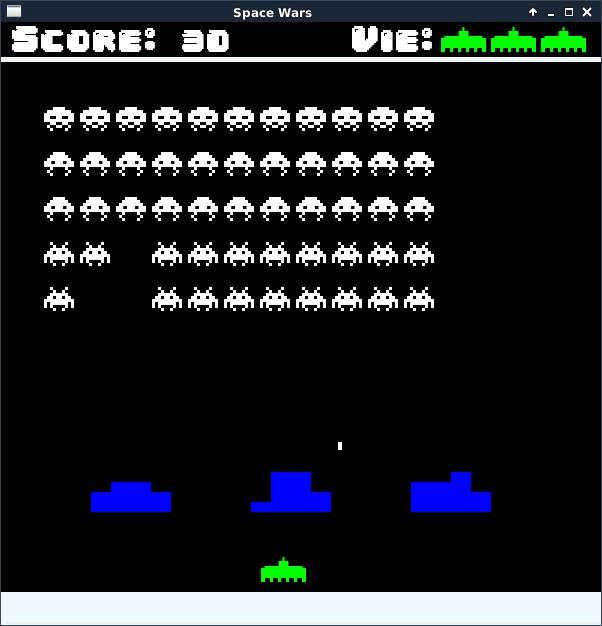
\includegraphics[width=0.55\linewidth]{JeuRealise}
	\end{center}
	Le jeu Space Wars en mode joueur contre joueur en réseaux aura la même interface graphique, à l'unique différence qu'il y aura le score du joueur 2 affiché à côté du score du joueur 1.

	\section{Présentation technique}
		\subsubsection{Diagramme de classe}
			\begin{center}
				\centering
				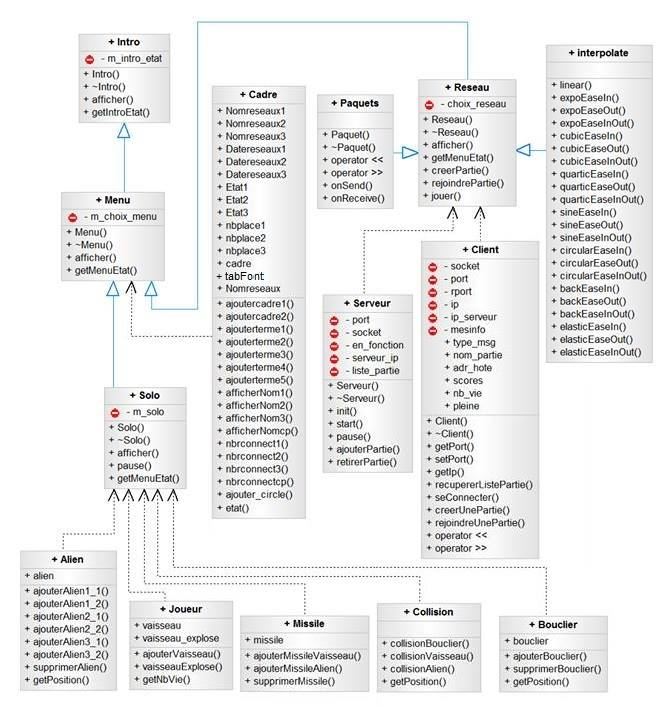
\includegraphics[width=1\linewidth]{Diagramme_de_classe}
%				\caption{Diagramme de classe}
			\end{center}
		\subsubsection{Diagramme de cas d'utilisation}
			\begin{center}
				\centering
				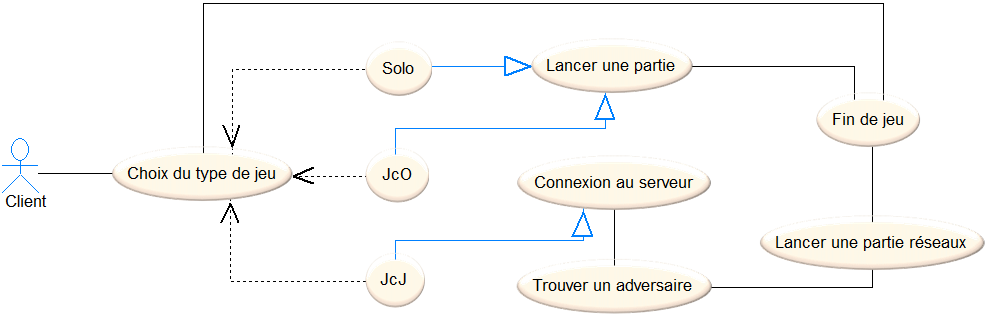
\includegraphics[width=0.8\linewidth]{DiagrammeDeCasDutilisation}
%				\caption{Diagramme de cas d'utilisation}
			\end{center}
		
		\subsection{Points importants}
			\subsubsection{Affichage}
				Nous avions comme contrainte d'utiliser la bibliothèque \textbf{SMFL} (\textbf{S}imple and \textbf{F}ast \textbf{M}ultimedia \textbf{L}ibrary) pour réaliser les interfaces graphiques du jeu.
				On a donc installé et utilisé les librairies via sfml-all.
				Nous avons utilisé des "Sprite" pour stocker nos images (alien, vaisseau, missile, bouclier), des textes avec différentes fonts pour afficher nos titres et nos informations (scores, vies, Nom du réseau, ...) et d'autres fonctionnalités de SFML pour créer les différentes interfaces graphiques.
				
			\subsubsection{Menu}
				Afin de gérer les différentes fonctionnalités du programme, un menu a donc été créé pour permettre à l'utilisateur de choisir la fonctionnalité du programme qui l'intéresse. Pour faire ce menu, on a donc créé au lancement de l'application une fenêtre de taille \textit{800x600} avec une petite introduction qui affiche le logo de la librairie \textbf{SMFL}. 
				Puis un menu apparaît suite à un effet de fondu. La classe Menu se base sur une variable qui passe d'un état à un autre. 
				Les différents états sont définis dans un \textsc{enum}. 
				La base de l'application est la classe Jeu qui gère les différents états du menu pour charger la classe approprié à l'état du Menu, en passant par référence la fenêtre pour l'affichage.
				
			
			\subsubsection{Jeu solo}
				Nous avons une classe solo qui utilise les classes bouclier, alien, vaisseau, joueur, collision et missile.
				Dans la classe solo, nous appelons toutes les classes nécessaire (celles ci-dessous) afin de gérer un jeu complet en solo.
				Dans la classe alien, nous gérons la création et l'élimination des aliens.
				Dans la classe bouclier, nous gérons l'ajout et la destruction de bouclier.
				Dans la classe joueur, nous gérons la vie, l'ajout et la destruction du joueur (vaisseau).
				Dans la classe collision, nous gérons toutes les collisions entre chaque entité.
				Dans la classe missile, nous gérons l'ajout et la suppression des missiles.
				
			\subsubsection{Réseau}
				Le jeu contient une partie jouable en réseau en temps réel. Nous connectons deux clients à un serveur qui sert de lien entre les deux clients. Chaque client communique avec le serveur via \textbf{UDP}. 
				Le serveur tient une liste des clients et une liste des parties. 
				Il est en charge de la transmission des informations à chacun des joueur d'une partie. Le serveur est donc une application extérieur au programme, qui est en charge de certaine fonctionnalités des parties en réseau. L'échange des données sur le réseau se fait via les paquets de la \textbf{SFML}.
						
			\subsubsection{État du produit à la fin du projet}
				Le produit (jeu) doit être fonctionnel à la fin du temps imparti, quitte à ne pas réaliser certaines fonctionnalités.
			\subsubsection{Portabilité}
				Le jeu doit être utilisable par toutes les distributions Linux à condition d'installer les packages suivants~:
				\begin{itemize}
					\item libsfml-dev
					\item libboost-dev
					\item pkg-config
				\end{itemize}
	\chapter{Bilan}
		\section{Déroulement du projet}
			\subsection{Prévisions}
				\begin{figure}[h]
					\centering	
					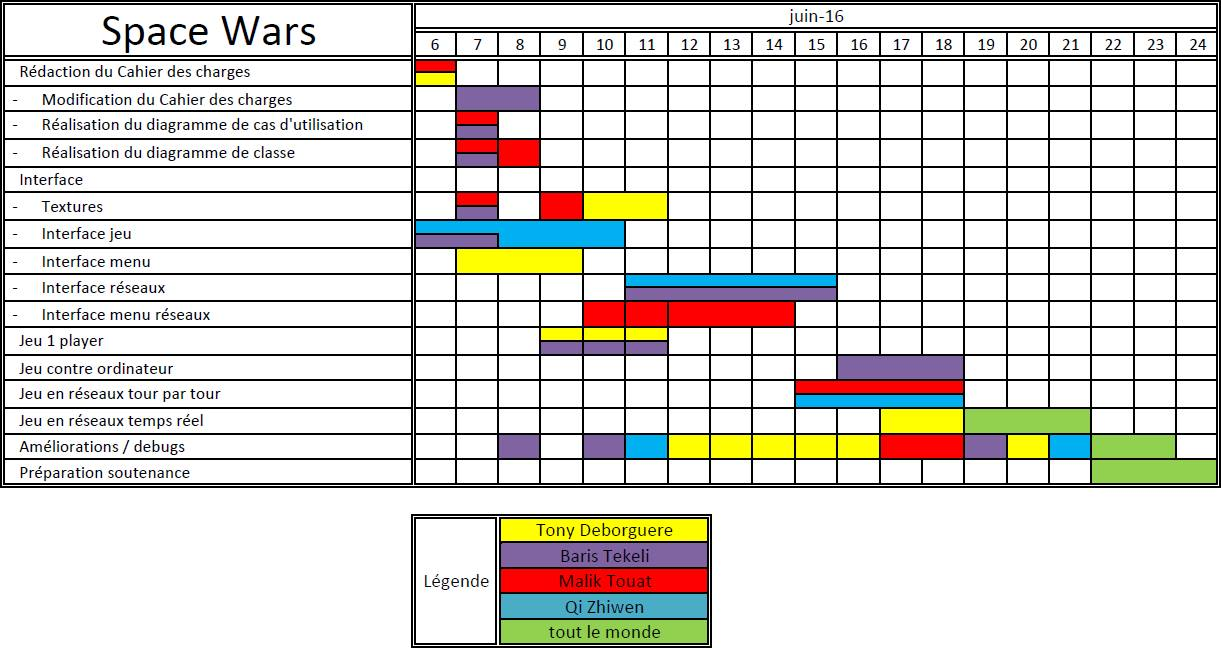
\includegraphics[width=1.05\linewidth]{PlanningPrevisionnel}
				\end{figure}		
				Comme indiqué sur le planning prévisionnel, nous avions prévu de finir le jeu solo assez tôt, de commencer l'IA, de faire le jeu en tour par tour et en temps réels en mettant le tout en réseau.
			\subsection{Problèmes rencontrés}
				\begin{description}
					\item[Problème 1] Le temps.
					\item[Problème 2] Compétences pour le réseau.
					\item[Problème 3] La gestion des événements avec la souris.
					\item[Problème 4] La gestion des collisions automatiques.
				\end{description}
			\subsection{Solutions}
			\begin{description}	
				\item[Problème 1] Nous avons décidé de ne pas faire tout ce que nous avions prévu:
				\begin{itemize}
					\item Nous avons fait un mode de jeu solo.
					\item Nous avons fait un mode de jeu en joueur contre joueur tour par tour
				\end{itemize}
				\item[Problème 2] Nous avons fait en sorte de faire des recherches sur internet et de commencer la partie réseaux dès le début du projet afin de mettre toutes les chances de notre côté. % à remplir
				\item[Problème 3] Pour gérer la souris, on finalement utiliser les fonctions de la SFML qui nous donne la taille d'un texte ou d'un sprite pour gérer ensuite la position de la souris par rapport à ces tailles
				\item[Problème 4] Nous avons dû faire une classe Collision avec une fonction pour chaque collision entre les différentes entités.
			\end{description}								
			
		\section{Conclusion (pour les projets futurs)}
			\subsection{Gestion des tâches à accomplir}
				Nous avons attribué à chaque membre de notre groupe les tâches à accomplir dans lesquels ils étaient les \textbf{meilleurs} afin d'être le plus efficace possible.
				Ayant personne de doué en réseau, nous avons attendu avant de commencer cette partie, et nous avons encore perdu du temps à faire des recherches sur internet.
			\subsection{Ce que nous a apporté ce projet}
				Nous avons fait quelques erreurs, comme la gestion du temps.
				C'est pourquoi, pour les prochains projets, nous devrons avoir de meilleures \textbf{prévisions} afin d'être sûr de pouvoir finir le projet.
				
				Nous savons mieux magner le langage C++, notamment avec la librairie SFML que nos avons utilisée lors de ces 3 dernières semaines.

		\section{Ressources}
			 Vous pouvez récupérer le logiciel ainsi que les ressources de celui-ci sur ce lien:
			 \begin{description}
			 	\item \href{https://github.com/l3info-MBT/Space_Wars}{https://github.com/l3info-MBT/Space\_Wars}
			 \end{description}
			 
			 Vous trouverez sur ce lien des informations supplémentaires sur la bibliothèque SFML:
			 \begin{description}
			 	\item
			 	\href{http://www.sfml-dev.org/index-fr.php}{http://www.sfml-dev.org/index-fr.php}
			 \end{description}
			 
			 Enfin, vous trouverez sur ce dernier lien les images et les sons qui nous ont servi dans la réalisation du jeu:
			 \begin{description}
			 	\item
			 	\href{http://www.classicgaming.cc/classics/space-invaders/}{http://www.classicgaming.cc/classics/space-invaders/}
			 \end{description}
			 
\end{document}